\documentclass[tikz,border=3mm]{standalone}
\usepackage[T1]{fontenc}
\usepackage{helvet}
\renewcommand{\familydefault}{\sfdefault}
\usepackage{amsmath,amssymb}
\usepackage{tikz}
\usetikzlibrary{shapes.geometric, positioning, decorations.pathreplacing,
                arrows.meta, calc, fit, backgrounds}

\begin{document}
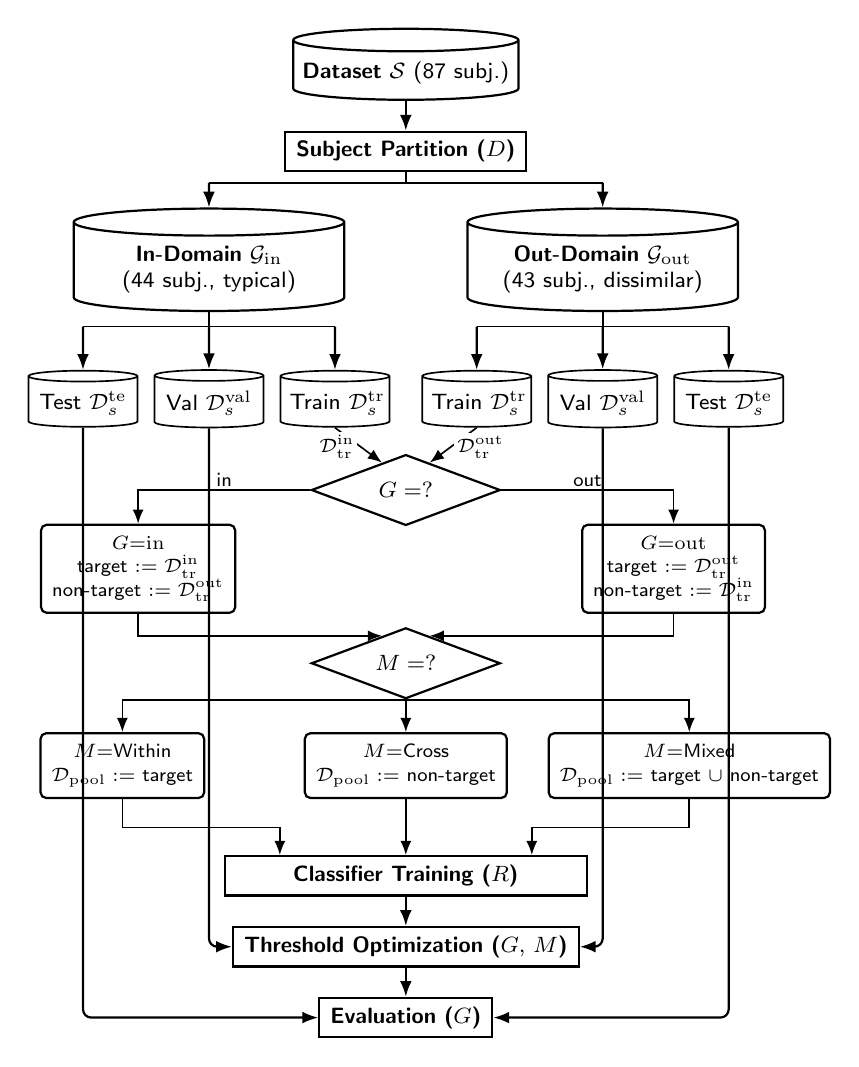
\begin{tikzpicture}[
  every node/.style={font=\sffamily\footnotesize},
  >=Latex,
  db/.style={draw, thick, cylinder, cylinder uses custom fill,
    cylinder body fill=white, shape border rotate=90, aspect=0.10,
    minimum width=2.6cm, minimum height=0.7cm, align=center,
    font=\sffamily\footnotesize},
  dbsm/.style={draw, semithick, cylinder, cylinder uses custom fill,
    cylinder body fill=white, shape border rotate=90, aspect=0.10,
    minimum width=1.35cm, minimum height=0.5cm, text width=1.15cm,
    align=center, font=\sffamily\footnotesize},
  pbox/.style={draw, thick,
    align=center, fill=white,
    minimum height=0.5cm,
    inner xsep=4pt, inner ysep=2pt,
    font=\sffamily\footnotesize},
  decision/.style={draw, thick, diamond, aspect=2.4, inner sep=1pt,
    fill=white, align=center, font=\sffamily\footnotesize},
  swbox/.style={draw, thick, rounded corners=2pt, align=center,
    fill=white, inner sep=4pt, font=\sffamily\footnotesize},
  arr/.style ={-{Latex[length=2mm, width=1.5mm]}, thick},
  arrsel/.style ={-{Latex[length=1.8mm, width=1.4mm]}, semithick},
  arrgated/.style={-{Latex[length=1.8mm, width=1.4mm]}, semithick, dashed},
  edgelbl/.style={font=\sffamily\scriptsize, inner sep=1pt, fill=white},
]

%% =========================================================
%% UPPER HALF — data partitioning
%% =========================================================
\node[db] (dataset) at (0,0)
  {\textbf{Dataset}~$\mathcal{S}$ (87 subj.)};

\node[pbox] (dsplit) at (0,-1.00)
  {\textbf{Subject Partition ($D$)}};
\draw[arr] (dataset.south) -- (dsplit.north);

\node[db, text width=3.2cm] (src) at (-2.5,-2.5)
  {\textbf{In-Domain} $\mathcal{G}_{\mathrm{in}}$\\(44 subj., typical)};
\node[db, text width=3.2cm] (tgt) at ( 2.5,-2.5)
  {\textbf{Out-Domain} $\mathcal{G}_{\mathrm{out}}$\\(43 subj., dissimilar)};

\coordinate (forkMid) at ($(dsplit.south)!.3!(src.north)$);
\coordinate (forkC) at (0,0 |- forkMid);
\coordinate (forkL) at (-2.5,0 |- forkMid);
\coordinate (forkR) at ( 2.5,0 |- forkMid);
\draw[thick] (dsplit.south) -- (forkC);
\draw[thick] (forkL) -- (forkR);
\draw[arr] (forkL) -- (src.north);
\draw[arr] (forkR) -- (tgt.north);

\node[dbsm] (test_s)  at (-4.1,-4.2) {Test~$\mathcal{D}_s^{\mathrm{te}}$};
\node[dbsm] (val_s)   at (-2.5,-4.2) {Val~$\mathcal{D}_s^{\mathrm{val}}$};
\node[dbsm] (train_s) at (-0.9,-4.2) {Train~$\mathcal{D}_s^{\mathrm{tr}}$};

\coordinate (forkS) at ($(src.south)!.25!(test_s.north)$);
\draw[semithick] (src.south) -- (-2.5,0 |- forkS);
\draw[semithick] (-4.1,0 |- forkS) -- (-0.9,0 |- forkS);
\draw[arr] (-4.1,0 |- forkS) -- (test_s.north);
\draw[arr] (-2.5,0 |- forkS) -- (val_s.north);
\draw[arr] (-0.9,0 |- forkS) -- (train_s.north);

\node[dbsm] (train_t) at (0.9,-4.2)  {Train~$\mathcal{D}_s^{\mathrm{tr}}$};
\node[dbsm] (val_t)   at (2.5,-4.2)  {Val~$\mathcal{D}_s^{\mathrm{val}}$};
\node[dbsm] (test_t)  at (4.1,-4.2)  {Test~$\mathcal{D}_s^{\mathrm{te}}$};

\coordinate (forkT) at ($(tgt.south)!.25!(test_t.north)$);
\draw[semithick] (tgt.south) -- (2.5,0 |- forkT);
\draw[semithick] (0.9,0 |- forkT) -- (4.1,0 |- forkT);
\draw[arr] (0.9,0 |- forkT) -- (train_t.north);
\draw[arr] (2.5,0 |- forkT) -- (val_t.north);
\draw[arr] (4.1,0 |- forkT) -- (test_t.north);

%% =========================================================
%% LOWER HALF — explicit (G, M) conditional routing
%% =========================================================

%% ---- G decision: which group is the evaluation target? ----
%% Branches relabel the two Train cylinders as Train_target / Train_non-target
%% via signals carried by the dashed arrows below.
\node[decision, minimum width=2.4cm, minimum height=0.9cm] (Gdec) at (0,-5.30)
  {$G = ?$};
\draw[arrsel] (train_s.south) -- ($(Gdec.north west)!0.5!(Gdec.north)$)
  node[edgelbl, pos=0.55, left=1pt] {$\mathcal{D}_{\mathrm{tr}}^{\mathrm{in}}$};
\draw[arrsel] (train_t.south) -- ($(Gdec.north east)!0.5!(Gdec.north)$)
  node[edgelbl, pos=0.55, right=1pt] {$\mathcal{D}_{\mathrm{tr}}^{\mathrm{out}}$};

%% G's two outgoing branches: relabel target / non-target.
%% G = in:  target = in,  non-target = out
%% G = out: target = out, non-target = in
\node[swbox, align=center] (Gin)  at (-3.4,-6.30)
  {\scriptsize $G{=}\mathrm{in}$\\[-1pt]
   \scriptsize target $:= \mathcal{D}_{\mathrm{tr}}^{\mathrm{in}}$\\[-1pt]
   \scriptsize non-target $:= \mathcal{D}_{\mathrm{tr}}^{\mathrm{out}}$};
\node[swbox, align=center] (Gout) at ( 3.4,-6.30)
  {\scriptsize $G{=}\mathrm{out}$\\[-1pt]
   \scriptsize target $:= \mathcal{D}_{\mathrm{tr}}^{\mathrm{out}}$\\[-1pt]
   \scriptsize non-target $:= \mathcal{D}_{\mathrm{tr}}^{\mathrm{in}}$};
\draw[arrsel] (Gdec.west) -| (Gin.north)
  node[edgelbl, pos=0.25, above] {in};
\draw[arrsel] (Gdec.east) -| (Gout.north)
  node[edgelbl, pos=0.25, above] {out};

%% ---- M decision: which subset of {target, non-target} is used for training? ----
\node[decision, minimum width=2.4cm, minimum height=0.9cm] (Mdec) at (0,-7.50)
  {$M = ?$};

%% Both G branches feed into M-decision (carrying the target / non-target labels).
\draw[arrsel] (Gin.south)  |- ($(Mdec.north west)!0.5!(Mdec.north)$);
\draw[arrsel] (Gout.south) |- ($(Mdec.north east)!0.5!(Mdec.north)$);

%% Three M-outputs: explicit selection rules
\node[swbox, align=center] (Mwithin) at (-3.6,-8.80)
  {\scriptsize $M{=}\text{Within}$\\[-1pt]
   \scriptsize $\mathcal{D}_{\mathrm{pool}} := $ target};
\node[swbox, align=center] (Mcross)  at ( 0.0,-8.80)
  {\scriptsize $M{=}\text{Cross}$\\[-1pt]
   \scriptsize $\mathcal{D}_{\mathrm{pool}} := $ non-target};
\node[swbox, align=center] (Mmixed)  at ( 3.6,-8.80)
  {\scriptsize $M{=}\text{Mixed}$\\[-1pt]
   \scriptsize $\mathcal{D}_{\mathrm{pool}} := $ target $\cup$ non-target};
\draw[arrsel] (Mdec.south) -| (Mwithin.north);
\draw[arrsel] (Mdec.south) -- (Mcross.north);
\draw[arrsel] (Mdec.south) -| (Mmixed.north);

%% ---- Merge the three M-branches into the rebalancing block ----
\node[pbox, minimum width=4.6cm] (cls) at (0,-10.20)
  {\textbf{Classifier Training}~\textbf{($R$)}};
\draw[arrsel] (Mwithin.south) |- ($(cls.north) + (-1.6,0.35)$) -- ++(0,-0.35);
\draw[arrsel] (Mcross.south)  -- (cls.north);
\draw[arrsel] (Mmixed.south)  |- ($(cls.north) + (1.6,0.35)$) -- ++(0,-0.35);

%% ---- Threshold Optimization ----
\node[pbox] (thr) at (0,-11.10)
  {\textbf{Threshold Optimization}~\textbf{($G,\,M$)}};
\draw[arr] (cls.south) -- (thr.north);

%% ---- Evaluation ----
\node[pbox] (eval) at (0,-12.00)
  {\textbf{Evaluation}~\textbf{($G$)}};
\draw[arr] (thr.south) -- (eval.north);

%% ---- Val / Test trunks (target side determined by G) ----
%% Both Val/Test cylinders feed Threshold/Evaluation; the active side is
%% selected by G consistent with the target choice above.
\draw[arr, rounded corners=3pt]
  (val_s.south) -- (-2.5,-11.10) -- (thr.west);
\draw[arr, rounded corners=3pt]
  (val_t.south) -- ( 2.5,-11.10) -- (thr.east);
\draw[arr, rounded corners=3pt]
  (test_s.south) -- (-4.1,-12.00) -- (eval.west);
\draw[arr, rounded corners=3pt]
  (test_t.south) -- ( 4.1,-12.00) -- (eval.east);

\end{tikzpicture}
\end{document}
